% \documentclass{article}
% % \usepackage[utf8]{inputenc}
% \usepackage{fullpage}
% \usepackage {setspace}
% \usepackage[hang,flushmargin]{footmisc} %control footnote indent
% \usepackage{url} % for Appendicessite links
% \usepackage{amssymb,amsmath}%for matrix
% \usepackage{graphicx}%for figure
% \usepackage{appendix}%for appendix
% \usepackage{float}
% \usepackage{multirow}
% \usepackage{longtable}
% \usepackage{morefloats}%in case there are too many float tables and figures
% \usepackage{caption}
% \usepackage{subcaption}
% \usepackage{listings}
% \captionsetup[subtable]{font=normal}
% \usepackage{color}
% \usepackage{hyperref}
% \usepackage[round]{natbib}
% \usepackage[export]{adjustbox}
% %\usepackage{Sweave}
% \setlength{\parindent}{0em}
% \setlength{\parskip}{0.5em}


% \graphicspath{{0.plots/}}


% \begin{document}
\subsection{Application}\label{sec:data}

%%%% briefly talk about which data will be used then talk about clinical background of HD
\subsubsection{The Predictors of Huntington's Disease (PREDICT-HD) Study}\label{sec:data_analysis}
The motivating PREDICT-HD study is an observational study that aims to identify the earliest signs of HD onset so that future HD drug trials can be targeted toward treatment that may slow the progression of the disease, or prevent it altogether \citep{paulsen2008detection}. Briefly, HD is known to be caused by the mutation of the first exon of the Huntington (HTT) gene, where expansion of the cytosine-adenine-guanine (CAG) is observed for HD patients.\par

%%%% More details on the PREDICT-HD study and the data set: longitudinal part and time-to-event part
The study recruited participants from 33 medical centers in six countries (i.e., USA, Canada, Germany, Australia, Spain, and UK) starting from August, 2002. Qualified participants were healthy pre-HD people without any symptoms of HD; i.e., who have not had a motor diagnosis of HD based on the Unified Huntington Disease Rating Scale (UHDRS) and had more than 35 HTT CAG repeats. Detailed inclusion and exclusion criteria can be found in \cite{paulsen2006preparing}. Baseline demographic information such as age, gender, education years, as well as clinical variables such as CAG repeat length and Beck Depression Inventory were recorded at enrollment. A total of 40 longitudinal biomarkers from five domains (i.e., motor, cognitive, psychiatric, functional, and imaging) were recorded. The data used in the current study contains 1078 individuals enrolled until July, 2014. Among those 1078 participants, 64\% are female and the mean age at baseline is 39.8 years (SD=10.39, range 18.1-83.7), education is 14.5 years (SD=2.60, range 8.0-20.0), and number of CAG repeats is 42.5 (SD=2.69, range 12-62). In this study, the time variable is defined as months since enrollment. The average follow-up time is 61.2 months (SD=39.6; range 0.12-144.0) and 959 (89\%) participants have data for at least two years. The survival event of interest is motor diagnosis of HD since enrollment, which is defined as having a diagnostic confidence level (DCL) score of 4 (the highest score)\citep{paulsen2014prediction}. During the study follow-up, 225 (21\%) events (HD onsets) were observed.



%%%% put demographic table here
% Table~\ref{tab:data} summaries the baseline demographics of the study cohort.

% \begin{table}[H]
% \centering
% \caption{Baseline demographics of the study cohort \citep{paulsen2014prediction}}
% \label{tab:data}
% \begin{adjustbox}{width=\textwidth,totalheight=\textheight,keepaspectratio}
% \begin{tabular}{llp{5cm}p{5cm}}
% \hline
%  Variable & Study cohort & Participants not diagnosed with HD during the study (n=835) & Participants diagnosed with HD during the study (n=225)\\
%  \hline
%  Women & 687(64\%) & 540(63\%) & 147(65\%)\\
%  Age (years) & 39.78(10.39) & 38.92(10.24)  & 43.03(10.31) \\
%  CAG repeat length & 42.49 (2.69)& 42.21(2.58)& 43.57(2.85)\\
%  CAP & 356.12(92.30) & 334.89(82.74)& 436.59(81.82)\\
%  Education (years) & 14.46(2.60)& 14.56(2.62) & 14.08(2.50)\\
%  Time in study (years) & 4.78(3.30)&  4.28(3.31) & 6.66(2.48)\\
%  \hline
% \end{tabular}
% \end{adjustbox}
% \end{table}

We select five longitudinal biomarkers, one from each domain, that are known to be strongly predictive of HD onset \citep{paulsen2014prediction} (see Appendices Section~3 for variable definitions). In the exploratory data analysis, we plot the scatter plots (with loess curves) and the kernel density plots of those selected variables (see Figure~\ref{fig:data_neurotot} and Appendices Figure~4). The distributions of TMS, {FrBe Executive Subscale} (FES), and {Total Functional Capacity} (TFC) all clearly deviate from normality, indicating a strong indication that the LMM may not be appropriate for these outcomes. From the loess curves, we observe the general direction of association between each longitudinal biomarker and the risk of HD onset. For example, {putamen} volume (intracranial-corrected) decreases over time and the brain atrophy from decreased putamen volume is associated with increased hazard of HD onset \cite{paulsen2014prediction}. To compare the longitudinal results on the same scale, we have standardized all longitudinal biomarkers.



We consider the following joint model for our data analysis:
\begin{equation*}\label{eqn:data_joint}
\left\{
\begin{array}{l}
y_{i}(t) = m_{it} + \varepsilon_{it} = \beta_0 + \beta_1 t+ \beta_2 age_{0i} + {u}_{i1} + u_{i2} t + \varepsilon_{i}(t),  \varepsilon_{i}(t)\sim ALD(0, \sigma, \tau)\\
h(T_i|\mathcal{M}_{iT_i};  \boldsymbol{\gamma}, \alpha) = \sum_{k=1}^3\lambda_kI_k(T_i)\exp(\gamma_1 education_i + \gamma_2 I_{male_i} + \alpha m_i(T_i))
\end{array}
\right.
\end{equation*}
where $y_{i}(t)$ represents one of the five selected longitudinal biomarkers and $age_i$ is the baseline age of subject $i$. In the survival sub-model, we specify a piecewise constant baseline hazard function with three time intervals, where $\lambda_k$ is the hazard rate for time interval $[t_k, t_{k+1})$ and $I_k(t)=1$ if $t\in[t_k, t_{k+1})$ and 0 otherwise.We have explored different numbers of time intervals and pieces and have obtained very similar results.

We randomly split the 1078 study participants into two datasets: a training dataset of 800 participants to draw statistical inference for the unknown parameters and a validation dataset of 278 participants for predictions of HD-free probability. In the model fitting step, two chains are initiated with diverse initial values and the chains are considered to converge if the potential scale reduction factors (PSRF) \citep{brooks1998general} for all parameters are below 1.1. In the prediction step we choose different censoring time ($t$) and prediction time window ($\Delta t$) combinations (similar to those chosen in the simulation study). Predictive accuracy for the test cohort is summarized using AUC, AARD ,and MRD defined in Section~\ref{sec:pred_accuracy} for each ($t, \Delta t$) combination as well as for each quantile in the QRJM. We also calculate the AUCs from the LMJM and compare them with those from our QRJM model.



\subsubsection{Inference Results for PREDICT-HD data}\label{sec:data_results}
Table~\ref{p1realdata_inference} (for the outcome TMS) and Appendices Table 4 (for the outcomes putamen, stroop word, FES, and TFC) present the inference results from the QRJMs at $\tau=$ 0.25, 0.50, and 0.75. In the longitudinal process, the coefficient for time quantifies the change rate of a specific longitudinal biomarker at a fixed quantile. For example, Table~\ref{p1realdata_inference} suggests that the time effect is 0.019 (95\% CI: 0.015, 0.023) for TMS at $\tau=0.25$, indicating one month increase in time is associated with 0.019 unit increase of TMS (when $\tau=0.25$). The positive time coefficients for TMS at all quantiles indicate that TMS increases (deteriorates) over time, which is consistent with the loess curves in Figure~\ref{fig:data_neurotot}. The magnitude of the time coefficient is similar at different quantiles for TMS, putamen, stroop word, and FES, indicating comparable progression in each of these outcomes at those quantiles. However, some variability is observed in TFC, where the time effect is highest at lower quantiles of TFC and becomes smaller at higher quantiles. Because lower TFC is associated with higher risk of HD onset, and these data indicate that the health of those with lower TFC deteriorates faster, special targeted care may be needed for those individuals in the lower quantile of TFC, in order to reduce their risk of HD onset.

Table~\ref{p1realdata_inference} also suggests that higher baseline age is associated with higher (worse) TMS and one year increase in baseline age is associated with 0.005 (95\% CI: 0.001, 0.010) units increase in TMS (when $\tau=0.5$). In the time-to-event process, across all three quantiles, education has protective effect on HD onset, i.e., those with more education years tend to have a lower risk of HD onset. Outcome TMS is strongly predictive of HD onset at all quantiles. Specifically, an unit increase in TMS increases the risk of HD onset by 4.600 ($\exp(1.526)$, 95\% CI 3.747-5.726) times at $\tau=0.25$, by 3.669 (95\% CI 3.152-4.302) times at $\tau=0.5$, and by 2.945 (95\% CI 2.633-2.294) times at $\tau=0.75$, respectively. Similarly, worse outcomes in putamen, stroop word task, FES, and TFC are also strongly associated with higher risk of HD onset across all quantiles.


% latex table generated in R 3.2.0 by xtable 1.8-0 package
% Mon Jan 11 22:29:09 2016
% \begin{table}[H]
% \centering
% \caption{Model estimations from QRJM with different quantiles of {Total motor score} in the longitudinal process.}
% \label{realdata_neurotot}
% \begin{tabular}{rrrrrr}
%   \hline
%  & Lower95 & Median & Upper95 & Mean & SD \\
%   \hline
%   \multicolumn{6}{c}{$\tau=0.25$}\\
%   \hline
%   \multicolumn{2}{l}{\textit{longitudinal process}} & & & &\\
%   int. & -0.652 & -0.614 & -0.574 & -0.614 & 0.020\\
%   time & 0.014 & 0.019 & 0.023 & 0.019 & 0.003\\
%   \multicolumn{2}{l}{\textit{time-to-event process}} & & & &\\
%   assoct. & 1.137 & 1.295 & 1.465 & 1.298 & 0.083 \\
%   eduyr & -0.124 & -0.093 & -0.068 & -0.095 & 0.015\\
%   % gamma2[1] & 0.000 & 0.000 & 0.000 & 0.000 & 0.000 &  \\
%   male & -0.040 & 0.335 & 0.715 & 0.333 & 0.193\\
%    \hline
%      \multicolumn{6}{c}{$\tau=0.50$}\\
%   \hline
%   \multicolumn{2}{l}{\textit{longitudinal process}} & & & &\\
%   int. & -0.364 & -0.317 & -0.270 & -0.317 & 0.024 \\
%   time & 0.015 & 0.020 & 0.024 & 0.020 & 0.002 \\
%   \multicolumn{2}{l}{\textit{time-to-event process}} & & & &\\
%   assoct. & 1.027 & 1.164 & 1.306 & 1.167 & 0.071 \\
%   eduyr & -0.154 & -0.124 & -0.099 & -0.125 & 0.014 \\
%   % gamma2[1] & 0.000 & 0.000 & 0.000 & 0.000 & 0.000 &  \\
%   male & -0.079 & 0.300 & 0.671 & 0.300 & 0.193 \\
%    \hline
%         \multicolumn{6}{c}{$\tau=0.75$}\\
%   \hline
%   \multicolumn{2}{l}{\textit{longitudinal process}} & & & &\\
%   int. & -0.050 & 0.007 & 0.062 & 0.007 & 0.028 \\
%   time & 0.016 & 0.021 & 0.025 & 0.021 & 0.002 \\
%   \multicolumn{2}{l}{\textit{time-to-event process}} & & & &\\
%   assoct. & 0.901 & 1.009 & 1.115 & 1.009 & 0.055 \\
%   eduyr & -0.174 & -0.145 & -0.119 & -0.146 & 0.014 \\
%   % gamma2[1] & 0.000 & 0.000 & 0.000 & 0.000 & 0.000 &  \\
%   male & -0.169 & 0.200 & 0.560 & 0.199 & 0.188\\
%    \hline
% \end{tabular}
% \end{table}


% \begin{sidewaystable}
\begin{table}[H]
\centering
\caption{PREDICT-HD data analysis: Parameter estimation and 95\% credible interval (in parenthesis) from QRJM at three different quantiles with TMS being the longitudinal biomarker.}
\label{p1realdata_inference}
\resizebox{\linewidth}{!}{
\begin{tabular}{lccc}
  \hline
  % & \multicolumn{3}{c}{{total motor score}}\\
  % \hline
  & $\tau=0.25$ & $\tau=0.50$ & $\tau=0.75$ \\
\hline
\multicolumn{4}{l}{For longitudinal TMS process}\\
Intercept & $-$0.760 ($-$0.903, $-$0.628)& $-$0.525 ($-$0.699, $-$0.359)& $-$0.249 ($-$0.469, $-$0.035)\\
Time (months) & 0.019 (0.015, 0.023)& 0.020 (0.016, 0.024)& 0.022 (0.018, 0.026)\\
Age & 0.004 (0.001, 0.008)& 0.005 (0.001, 0.010)& 0.006 (0.001, 0.012)\\ \\
\multicolumn{4}{l}{For time to HD onset process}\\
Education (years) & $-$0.083 ($-$0.115, $-$0.052)& $-$0.112 ($-$0.142, $-$0.082)& $-$0.128 ($-$0.157, $-$0.101)\\

Male & 0.317 ($-$0.037, 0.654)& 0.360 ($-$0.020, 0.708)& 0.317 ($-$0.010, 0.647)\\
association & 1.526 (1.321, 1.745)& 1.300 (1.148, 1.459)& 1.080 (0.968, 1.192)\\
  \hline
\end{tabular}
}
\end{table}
% \end{sidewaystable}

\subsubsection{Dynamic Predictions of HD Risk}\label{sec:data_pred}
To evaluate the predictive accuracy of the model, we make out-of-sample predictions using the test dataset. Results are summarized in Table~\ref{tab:data_auc} with a column of the AUC from prediction using the LMJM. There are several interesting ``patterns'' observed in Table~\ref{tab:data_auc}. First, for a fixed censoring time $t$, all summary statistics increase with the increase in $\Delta t$ (this is sensible in that HD-free probability decreases with time, thus it is easier for the model to differentiate those who will versus those who will not experience the event at later time points). Second, for the same $t+\Delta t$ value, we see an increase in all three statistics from $t=12$ months to $24$ months (e.g., $t=12, \Delta t = 24$ v.s. $t=24, \Delta t=12$) followed by comparable statistics (a slight decrease in MRD) from $t=24$ months to $48$ months (e.g., $t=24, \Delta t= 36$ v.s. $t=48, \Delta t=12$). The improvement in predictive performance can be due to the additional longitudinal data with increasing censoring time $t$. However, longer follow-up time leads to smaller sample size due to event occurrence and censoring. Similar findings are reported in the simulation. Third, compared with the LMJM, the QRJM has better prediction at some quantiles, but not all, because some quantiles of the outcome can be more informative in predicting future survival outcome than the conditional mean while some are not. There are also a few cases where the QRJM has better prediction at all quantiles ($t=48$ at all $\Delta t$) and vice versa ($t=24$, $\Delta t=24$).

\begin{table}[H]
\centering
\caption{PREDICT-HD data analysis: AUC, AARD and MRD of the predictions of HD-free probability from QRJM and AUC from LMJM with TMS as the longitudinal biomarker.}
\label{tab:data_auc}
\adjustbox{max width=\textwidth}{
\begin{tabular}{rrrrrrrrrrrrrrc}
\hline
$t$ & $\Delta t$ & \multicolumn{3}{c}{AUC ($\tau$)} & & \multicolumn{3}{c}{AARD ($\tau$)} & & \multicolumn{3}{c}{MRD ($\tau$)} & & \multirow{2}{*}{AUC (LMJM)}\\
\cline{3-5}  \cline{7-9} \cline{11-13}
\multicolumn{2}{c}{(month)}  & 0.25 & 0.50 & 0.75 &  & 0.25 & 0.50 & 0.75&  & 0.25 & 0.50 & 0.75 & & \\
\hline
\multirow{3}{*}{$12$}  & 12 & 0.647 & 0.683 & 0.738 && 0.213 & 0.261 & 0.356 &&  0.010 & 0.020 & 0.059 & &0.679\\
            & 24 &  0.668 & 0.702 & 0.753 &&  0.244 & 0.290 & 0.379 && 0.028 & 0.054 & 0.128 && 0.695\\
            & 36 &  0.685 & 0.714 & 0.760 &&  0.273 & 0.311 & 0.391 && 0.054 & 0.091 & 0.170  & &0.693\\[0.5em]
\multirow{3}{*}{$24$}  & 12 & 0.836 & 0.857 & 0.864  && 0.539 & 0.575 & 0.577 &&  0.168 & 0.218 & 0.285 & &0.855\\
            & 24 &  0.852 & 0.872 & 0.873 && 0.566 & 0.598 & 0.583 && 0.285 & 0.361 & 0.404 & &0.878\\
            & 36 & 0.866 & 0.877 & 0.872 &&  0.581 & 0.599 & 0.575 && 0.368 & 0.420 & 0.430 & &0.836\\[0.5em]
\multirow{3}{*}{$48$}  & 12 &  0.875 & 0.878 & 0.868 &&  0.583 & 0.598 & 0.589 && 0.326 & 0.320 & 0.303 & &0.669\\
            & 24 & 0.875 & 0.883 & 0.874 && 0.578 & 0.602 & 0.598  &&  0.390 & 0.401 & 0.379 & &0.769\\
            & 36 &  0.877 & 0.887 & 0.879 && 0.589 & 0.614 & 0.599  && 0.417 & 0.439 & 0.417 & &0.774\\
\hline
\end{tabular}
}
\end{table}

We select three individuals (with IDs 12, 63, and 110) with different TMS trajectories (Figure~\ref{plot:datafig11}) to illustrate how our method provides subject-specific dynamic predictions of HD-free survival. For each individual, predictions are calculated and then updated based on increasing number of longitudinal measurements. In Figure~\ref{plot:datafig12}, we have the longitudinal measures up to 24 months ($t=24$) for each subject, and predictions are made for $\Delta t$ being 12, 24, 36, and 48 months respectively. We then increase the follow-up time to 36 and 48 months ($t=36$ and $t=48$) and update the predictions using the same $\Delta t$ values. Updated prediction results are displayed in Figure~\ref{plot:datafig13} ($t=36$) and Figure~\ref{plot:datafig14} ($t=48$), respectively. The plots suggest that participants with lower and stable TMS have much higher HD-free probability (i.e., lower predicted risk of HD onset, subject 12 v.s. subjects 62 and 110). With longer follow-up times and more longitudinal measurements, predicted HD-free probabilities are updated based on the entire longitudinal history and are more accurate as indicated by the narrower point-wise 95\% credible intervals as one looks at predictions from censoring time $t=24$ months down to $t=48$ months.

\begin{figure}[H]
\subfloat[Longitudinal trajectories of TMS for three selected subjects.]{
    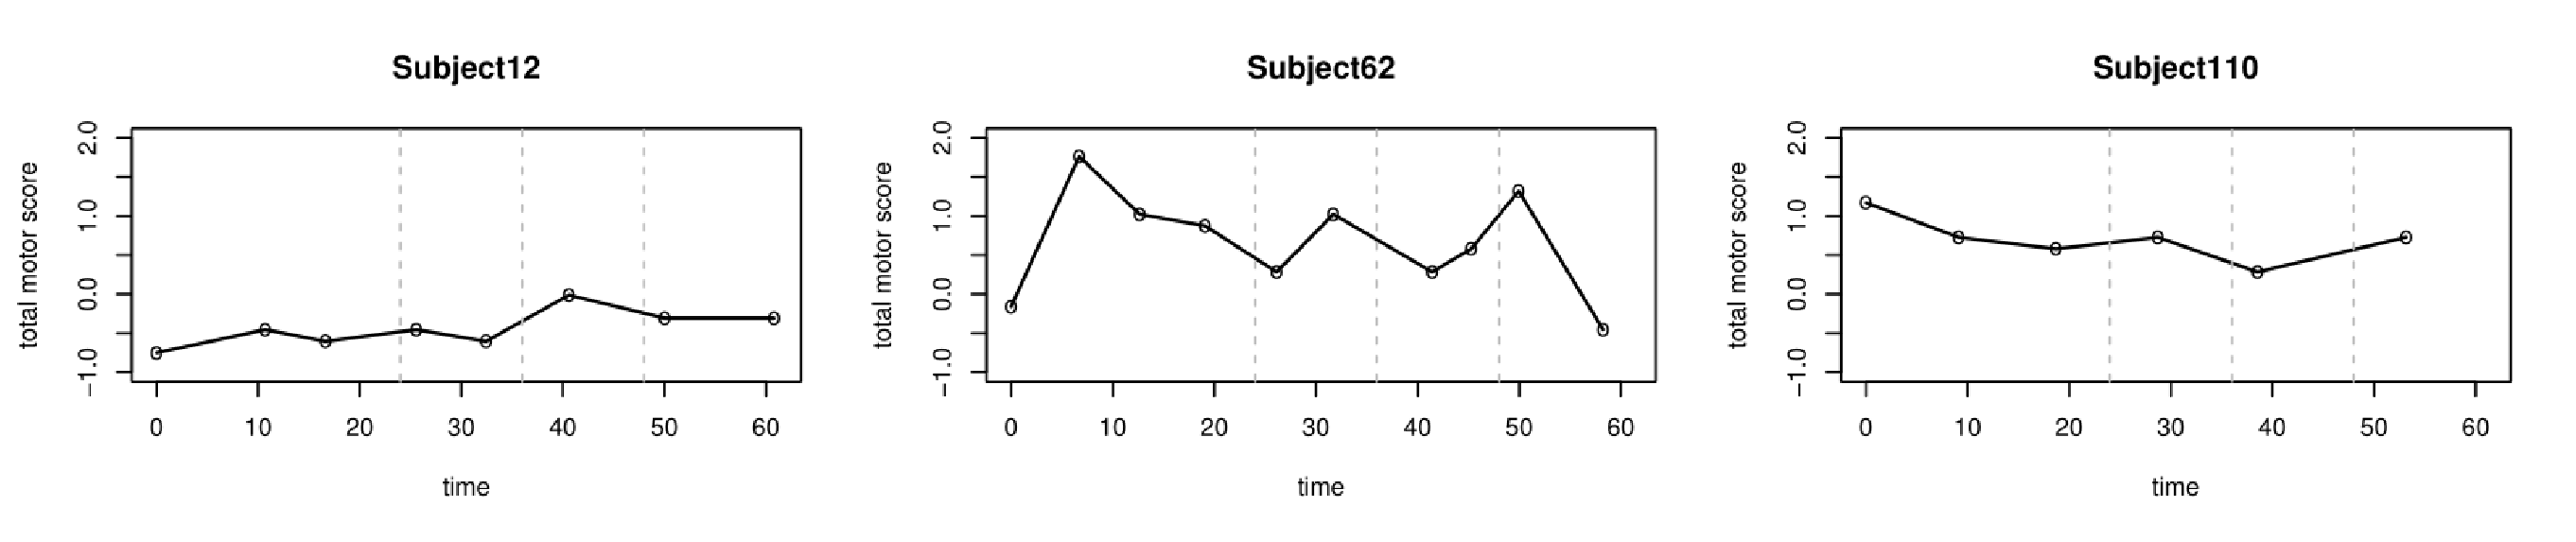
\includegraphics[width=\columnwidth]{test_long_plot_12_62_110.eps}\label{plot:datafig11}
}

% \centering
\subfloat[Predictions based on censoring time $t=$ 24 months]{
    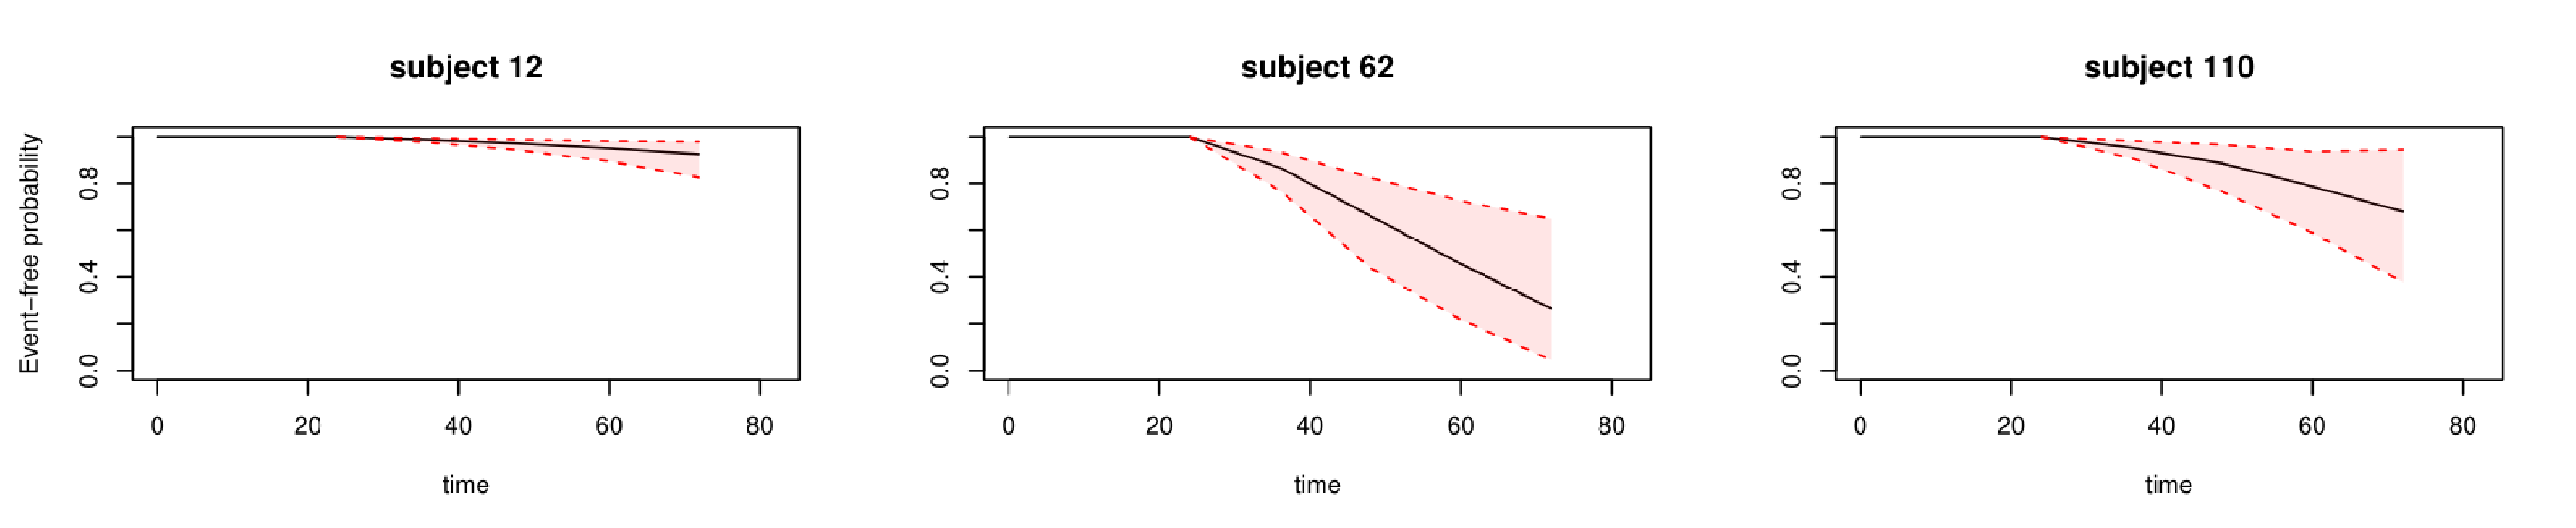
\includegraphics[width=\columnwidth]{neurotot_qt50_pred_surv_t24_id_12_62_110.eps}\label{plot:datafig12}
}

\subfloat[Predictions based on censoring time $t=$ 36 months]{
    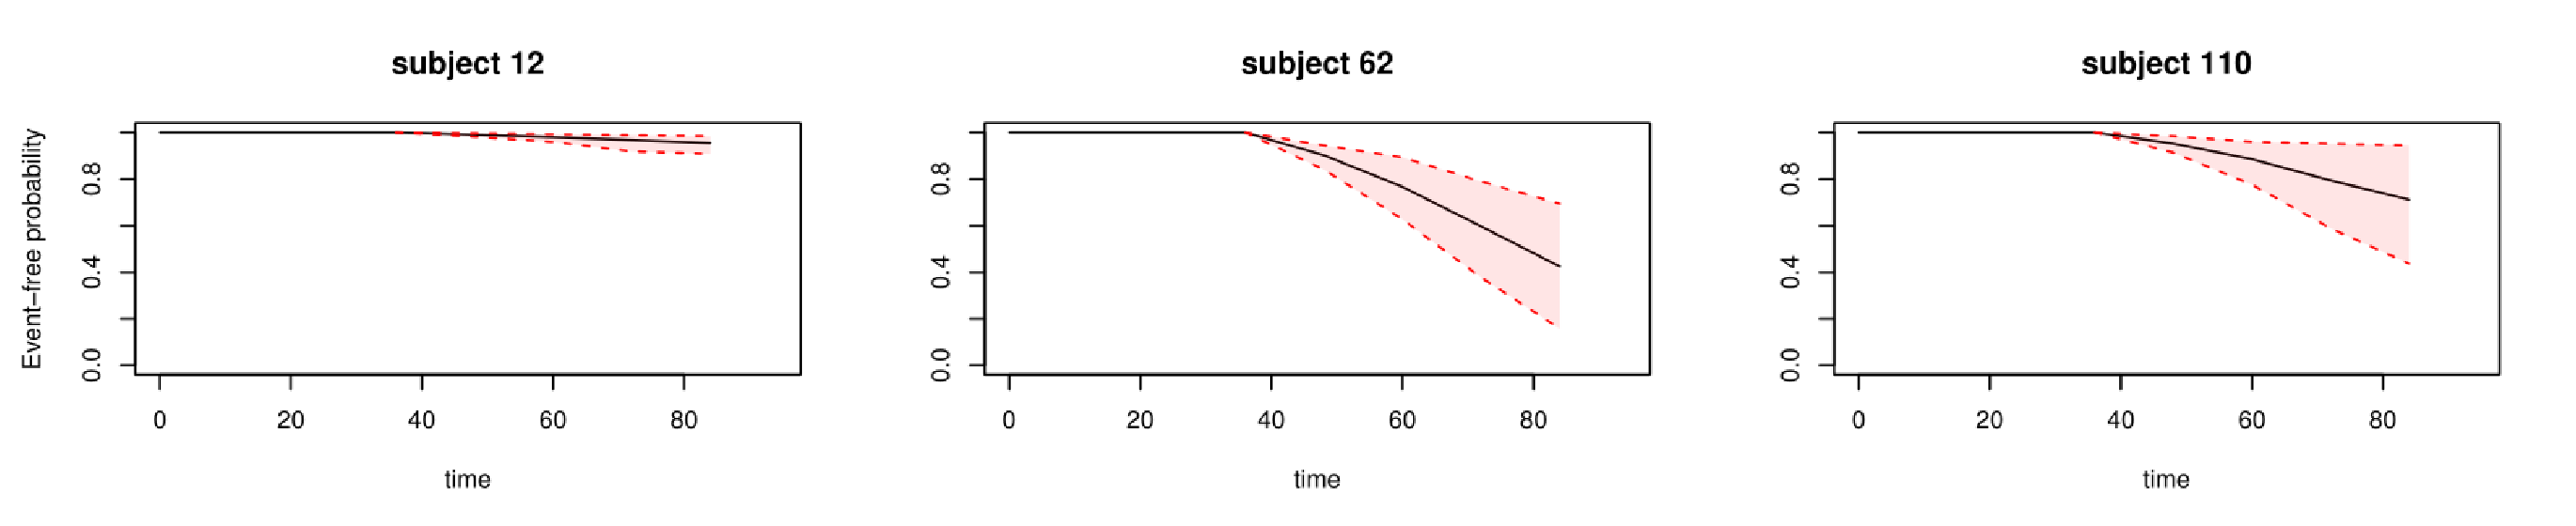
\includegraphics[width=\columnwidth]{neurotot_qt50_pred_surv_t36_id_12_62_110.eps}\label{plot:datafig13}
}

\subfloat[Predictions based on censoring time $t=$ 48 months]{
    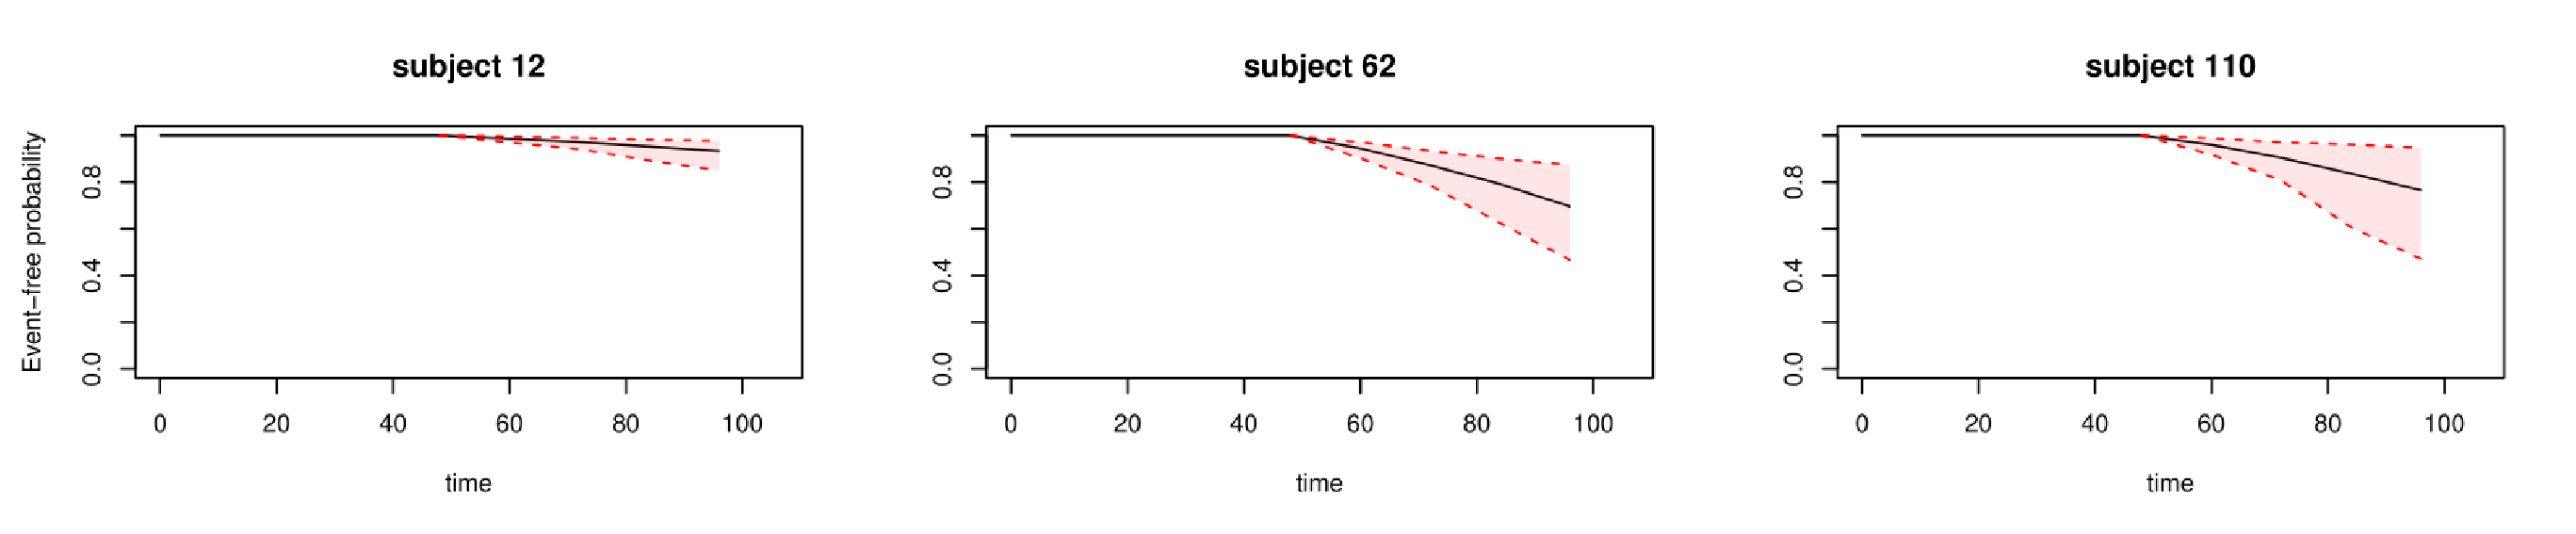
\includegraphics[width=\columnwidth]{neurotot_qt50_pred_surv_t48_id_12_62_110.eps}\label{plot:datafig14}
}

  \caption{PREDICT-HD data analysis: Longitudinal trajectories and dynamic predictions of HD-free probabilities with 95\% pointwise credible interval from QRJM at $\tau=0.5$ for selected subjects.}
  \label{plot:datafig1}
\end{figure}



% \end{document}
